\clearpage
\appendix
\section*{Technical Appendix}

\subsection*{Relation to Other Formalisms}
\paragraph*{$\mathsf{SFCL} < \CSL$}

We provide an argument for $\mathsf{SFCL}$ that extends the language of propositional logic with constructs $\langle \! \langle  C \rangle \! \rangle (\varphi;\psi_1,...,\psi_k)$ meaning that `coalition $C$ can achieve $\varphi$ while also enabling $\overline{C}$ to achieve any of $\psi_1,...,\psi_k$ (via a suitable joint action)'. 

Formally, the semantics is defined as 
\begin{gather*}
    \G,s \models \langle \! \langle C \rangle \! \rangle (\varphi; \psi_1, ..., \psi_k) \text{ iff }\\
    \exists \sigma_C (\forall \sigma_{\overline{C}} : \G,t \models \varphi \text{ and } \forall \psi_i, \exists  \sigma_{\overline{C}}:\G,u \models \psi) \text{ with } \\ t,u \in S \text{ s.t. } \langle s, \sigma_C \cup \sigma_{\overline{C}}, w \rangle \in R
\text{ and } w \in \{t,u\}.
\end{gather*}
\iffalse
  \begin{alignat*}{3}
        &\G,s \models \langle \! \langle C \rangle \! \rangle (\varphi; \psi_1, ..., \psi_k) && \text{ iff } && \exists \sigma_C (\forall \sigma_{\overline{C}} : \G,t \models \varphi \text{ and }\\ 
       & && && \forall \psi_i, \exists  \sigma_{\overline{C}}:\G_u \models \psi) \text{ with } \\
         & && &&  t,u \in S \text{ s.t. } \langle s, \sigma_C \cup \sigma_{\overline{C}}, w \rangle \in R\\
        & && && \text{ and } w \in \{t,u\}.   
\end{alignat*}   
\fi

Now, let us have another look at CGSs in Figure \ref{fig::exampleCGM}. Recall that these structures are distinguished by the $\CSL$ formula $\exists x \assign{x,x} \lnot p$. We claim that no formula of $\mathsf{SFCL}$ can distinguish $\G_1,s$ from $\G_2,s$. An informal sketch of the induction-based argument is as follows. For purely propositional formulas it is clear that $\G_1,w$ and $\G_2,w$ with $w\in \{s,t\}$ satisfy the same formulas. Now, let us consider socially-friendly coalitional modalities $\langle \! \langle  C \rangle \! \rangle (\varphi;\psi_1,...,\psi_k)$ For the case of grand coalition $C = \{1,2\}$, it is easy to verify that any move in $\G_1,w$ can be matched by a corresponding move $\G_2,w$ to satisfy $\varphi$. Clearly, these transitions will require different actions by agents, but since we do not have access to action labels in $\mathsf{SFCL}$, we are not able to spot the difference. 

For the case of single agents, observe that yet again, every choice of, let's say, agent 1 in one structure can be matched by a choice in the other structure to the same effect. Indeed, whatever agent 1 chooses in $\G_1, s$, $a$ or $b$, she can only satisfy some $\varphi$ that holds in both states $s$ and $t$ (due to the fact that the outcome is determined by what agent 2 chooses as well). Similarly in $\G_2, s$. Now, goals $\psi_i$ of agent 2 can either be satisfied in state $s$, state $t$, or both states. Hence, by the construction of CGSs, in both $\G_1$ and $\G_2$ for each choice of agent 1, agent 2 has an action to either stay in the current state or force the transition to another state. That the outcome of the corresponding transitions satisfy $\psi_i$ follows from the induction hypothesis. 
\newline
\newline
\textbf{Proposition 1.}  $\mathsf{AL}$ is not at least as expressive as $\CSL$.

\begin{proof}
  Consider $\exists x \assign{x, x} \lnot p \in \CSL$, and assume towards a contradiction that there is an equivalent $\varphi \in \mathsf{AL}$. Since we have a countably infinite set of constants $\mathcal{C}$ (and hence actions) at our disposal  and due to the fact that $\varphi$ is finite, we can assume that there are actions $a$ and $b$ that do not appear explicitly in $\varphi$. 

Now, consider two concurrent game structures defined over two agents and two actions in Figure \ref{fig::exampleCGM}. As we have already seen in our argument for Proposition \ref{prop:cslVScl}, $\G_1,s \models \exists x \assign{x, x} \lnot p$ and $\G_2,s \not \models \exists x \assign{x, x} \lnot p$. What is left to show is that $\varphi$ cannot distinguish the two structures, i.e. $\G_1,s \models \varphi$ if and only if $\G_2, s \models \varphi$. 

       The proof is by induction on the complexity of $\varphi$. As the \textit{Base Case}, by the construction of the structures we have that $\G_1,w \models p$ if and only if $\G_2,w \models p$ for $w \in \{s,t\}$ and all $p \in \Ap$. 

    \textit{Induction Hypothesis.} $\G_1,w \models \psi$ if and only if $\G_2, w \models \psi$  for $w \in \{s,t\}$ and for all strict subformulas $\psi$ of $\varphi$.
    
    Boolean cases follow straightforwardly by the induction hypothesis. What is left is the case of modality markers. 

   \textit{Case } $\varphi := [M]\psi$. First, recall that we assume that actions $a$ and $b$ do not appear explicitly in $\varphi$. It is enough to verify four forms of modality markers corresponding to all possible combinations of quantifiers over actions for two agents. Let $\varphi = [\exists x, \exists y] \psi$. It is easy to see that  $\G_1,w \models [\exists x, \exists y] \psi$ if and only if $\G_2,w \models [\exists x, \exists y] \psi$ as in both CGSs the grand coalition of agents $\{1,2\}$ has the full control over which transitions to force. Hence, each move in $\G_1,w$ to a $\psi$-state $v \in \{s,t\}$ can be matched by a move in  $\G_2,w$ to the same $\psi$-state $v$, where we will have $\G_1,v \models \psi$ if and only if $\G_2,v \models \psi$ by the induction hypothesis. 
   The remaining cases for modality markers can be shown similarly.
\end{proof}

\subsection*{Soundness and Completeness}

\textbf{Lemma 1.}
    Each axiom schema of $\CSL$ is valid and each rule of $\CSL$ preserves validity.%: if the premised of a rule are valid so it is its conclusion. 

\begin{proof}
 For the sake of simplicity, we only consider closed instances of the axiom schemata. Validity of other axiom schemata and the soundness of the rules of inference can be shown similarly.
 
 ($\mathsf{N}$). Suppose that $\G,s\models \neg \assign{\vec{{a}}}\varphi$. By the definition of the semantics, this means that $\G,s\not \models \assign{\vec{{a}}} \varphi$, i.e. for each   $t\in S$ if   $\tuple{s,\vec{a},t}\in R$,  then we have that $\G,t\not\models \varphi$. From the seriality and functionality of $R$, we can conclude that there is exactly one such $t$, and thus $\G,s\models \assign{\vec{{a}}}\neg \varphi $. For the converse direction, suppose that $\G,s\models \assign{\vec{{a}}}\neg \varphi$. This means that there is a $t$ such that $\tuple{s,\vec{a},t}\in R$ and $\G,t\not\models \varphi$. By functionality of $R$ there is no other $t$ related to $s$ by means of $\vec{a}$, and thus we can conclude that $\G,s\models \neg \assign{\vec{{a}}}\varphi$. 

 ($\mathsf{B}$). Assume that $\G,s \models \forall x \assign{\vec t} \varphi$, where $x$ is different from every $t_i$. Since the formula is closed, this is just $\G,s \models \forall x \assign{\vec{ {a}}} \varphi$ for some $\vec{a}\in \mathcal D$. By the truth definition, this is equivalent to $\G,s \models \assign{\vec{{a}}} (\varphi [{b}/x])$ for every $b\in \Ac$, which means $\G,s\models \assign{\vec{ a}} \forall x \varphi $.
%\begin{description}
 %   \item[($\mathsf{N}$)] Suppose that $\G,s\models \neg \assign{\vec{{a}}}\varphi$. By the definition of the semantics, this means that $\G,s\not \models \assign{\vec{{a}}} \varphi$, i.e. for each   $t\in S$ if   $\tuple{s,\vec{a},t}\in R$,  then we have that $\G,t\not\models \varphi$. From the seriality and functionality of $R$, we can conclude that there is exactly one such $t$, and thus $\G,s\models \assign{\vec{{a}}}\neg \varphi $. For the converse direction, suppose that $\G,s\models \assign{\vec{{a}}}\neg \varphi$, this means that there is an $t$ such that $\tuple{s,\vec{a},t}\in R$ and $\G,t\not\models \varphi$. By functionality of $R$ there is no other $t$ related to $s$ by means of $\vec{a}$, and thus we can conclude that $\G,s\models \neg \assign{\vec{{a}}}\varphi$. 
  %  \item[($\mathsf{B}$)] Assume that $\G,s \models \forall x \assign{\vec t} \varphi$, where $x$ is different from every $t_i$. Since the formula is closed, this is just $\G,s \models \forall x \assign{\vec{ {a}}} \varphi$ for some $\vec{a}\in \mathcal D$. By the truth definition, this is equivalent to $\G,s \models \assign{\vec{{a}}} (\varphi [{b}/x])$ for every $b\in \Ac$, which means $\G,s\models \assign{\vec{ a}} \forall x \varphi $. \qedhere 
%\end{description}
\end{proof}

\textbf{Lemma 2.}
    If $X$ is a consistent set of sentences over a given signature $\alpha$, then there is a consistent set of sentences $Y$ over $\alpha^\star$ such that $X\subseteq Y$, and $Y$ has the $\forall$-property.  


\begin{proof}
    Let $E$ be an enumeration of sentences of the form $\forall x \varphi$ over $\alpha^\star$. We define a sequence of sets of sentences $Y_0,Y_1,\ldots$ with $Y_0=X$ and $Y_{n+1}=Y_n \cup \set{ \varphi[a/x]\to \forall x \varphi}$ where $\forall x \varphi$ is the $n+1$-th sentence in $E$, and $a$ is the first constant in the enumeration occurring neither in $Y_n$ nor in $\varphi$. Since $Y_0$ is over $\alpha$, $Y_n$ is obtained by the addition of $n$ sentences over $\alpha^\star$, and $\alpha^\star$ includes a countably infinite set of new constants, we can always find such an $a$. 
    
    Now we show that $Y_{n+1}$ constructed in the described way is consistent. For this, assume towards a contradiction that $Y_n$ is consistent and $Y_{n+1}$ is not. This means that there is a finite set of sentences $U\subseteq Y_n$ such that $U\cup \set{\varphi [a/x]\to \forall x \varphi}\vdash \bot$. By the propositional reasoning we thus obtain that (i) $U\vdash \varphi [a/x]$ and (ii) $U\vdash \neg \forall x \varphi$. Since $a$ does not appear in $Y_n$, we can use the  $\mathsf{Gen}$ rule of inference and conclude that $U\vdash \forall x \varphi$. In conjunction with (ii) this amounts to the fact that $Y_n$ is not consistent, and hence we arrive at a contradiction.
    %and thus, because of (ii), that $U\vdash \bot$ which contradicts that $Y_n$ is consistent. 
    
    Define $Y$ as $\bigcup_{n\in \mathbb{N} }Y_n$. It is now easy to see that $Y$ is consistent and has the $\forall$-property. 
\end{proof}

\textbf{Proposition 6.}
    For all states $X, Y \in S^C$ %of the canonical model, 
    and for every decision $\vec{a} \in \mathcal{D}^C$, it holds that $\tuple{X,\vec{a},Y}\in R^C$ iff for every sentence $\varphi$, $\assign{\vec{a}}\varphi\in X $ implies $\varphi\in Y$

\begin{proof}
    Left-to-right: suppose $\tuple{X,\vec{a},Y}\in R^C$  and $\varphi\not\in Y$. We need to show that $\assign{\vec{a}}\varphi\notin X$. Since $Y$ is maximally consistent, we have that $\neg\varphi\in Y$. From the fact that $\tuple{X\,\vec{a},Y} \in R^C$ it follows, by Definition \ref{def:can_model}, that $\assign{\vec a}\neg \varphi\in X$. Since $X$ is maximally consistent, we have that $\neg\assign{\vec a} \neg \varphi \not\in  X$, which implies, by axiom $\mathsf{N}$, that $\assign{\vec{a}}\varphi\notin X$. 
    
    Right-to-left: we again reason by contraposition. Suppose that $\tuple{X,\vec{a},Y}\notin R^C$, and thus, by the construction of the canonical model, there is a formula $\varphi \in Y$ such that $\assign{\vec a}\varphi\notin X$. Since $X$ is maximally consistent,  we have that $\neg\assign{\vec a}\varphi\in X$. By the axiom $\mathsf{N}$ we get $\assign{\vec{a}}\neg \varphi \in X$. Thus $\assign{\vec{a}}\neg \varphi \in X$ and $\neg\varphi \not\in Y$ as required for the proof. 
\end{proof}

\textbf{Proposition 7.} The canonical model $\G^C$ is a CGS.

\begin{proof}
    We have to prove that the relation $R^C$ of the canonical model is serial and functional. 
    
    For seriality, we have that given any state $X \in S^C$, %of the canonical model, 
    $X$ contains the formula $\assign{\vec{a}}\top$ for any $a\in D^\mathcal{C}$ %because $\top $ is a tautology and because of rule $\mathsf{Gen}$.
    due to $\top$ being a tautology and the application of $\mathsf{Nec}$.
    Thus, by Lemma \ref{lemma:lindy}, for any $\vec{a}\in D^C$ there is a $Y\in S^C$ such that $\set{\top}\cup \set{\psi \mid  \assign{\vec a} \psi\in X} \subseteq Y $, and by Proposition \ref{prop:existforall} we have that $\tuple{X,\vec{a},Y}\in R^C$

    For functionality, suppose that $\tuple{X,\vec{a},Y}\in R^C$, $\tuple{X,\vec{a},Z}\in R^C$ and $Z\neq Y$. Thus there is a $\varphi$, such that $\varphi\in Y$ and $\neg \varphi \in Z$. By the definition of $R^C$, this implies $\assign{\vec{a}}\varphi \in X$ and $\assign{\vec a} \neg \varphi \in X$.
    By $\mathsf{N}$, the latter is equivalent to $\neg \assign{\vec a}\varphi \in X$, which contradicts the consistency of $X$.
    %and by axiom $\mathsf{N}$ and $\mathsf{MP}$ that $\neg \assign{\vec a}\varphi \in X$ against the consistency of $X$. 
\end{proof}

\subsection*{Model Checking}
Full model checking algorithm for $\CSL$ and the \textit{PSPACE}-hardness proof (see Algorithm \ref{cslMCfull}).
\begin{algorithm}
	\caption{An algorithm for model checking $\CSL$} \label{cslMCfull} 
	\small
 %\footnotesize
	\begin{algorithmic}[1] 		
		\Procedure{MC}{$\G, s, \varphi$}		
      \Case {$\varphi = p$}
            \State{\textbf{return} $s \in \mathcal{V}(p)$}
        \EndCase
          \Case {$\varphi = \lnot p$}
            \State{\textbf{return} not $s \in \mathcal{V}(p)$}
        \EndCase
       \Case {$\varphi = \psi \lor \chi$}
            \State{\textbf{guess} $\theta \in \{\psi, \chi\}$  }
            \State{\textbf{return} $\textsc{MC} (\G,s,\theta)$}
        \EndCase
               \Case {$\varphi = \psi \land \chi$}
            \State{\textbf{universally choose} $\theta \in \{\psi, \chi\}$  }
            \State{\textbf{return} $\textsc{MC} (\G,s,\theta)$}
        \EndCase
       \Case {$\varphi = \assign{a_1,...,a_n} \psi$}
       \State{\textbf{guess} $t \in S$ such that   $\tuple{s, a_1, ..., a_n, t} \in R$}
       \State{\textbf{return} $\textsc{MC} (\G, t, \psi)$}
       %%\If {$\tuple{s, a_1, ..., a_n, t} \in R$ for some $t\in S$}
            %\State{\textbf{return} $\textsc{MC} (\G, t, \psi)$}
        %\Else
       %     \State{\textbf{return} \textit{false}}
      % \EndIf
       %     \State{\textbf{return} $\textsc{MC} (\G,s,\psi)$ or  $\textsc{MC} (\G,s,\chi)$}
        \EndCase
         \Case{$\varphi = \exists x \psi$}
        \State{\textbf{guess} $a \in \Ac$  }
        \State{\textbf{return} $\textsc{MC} (\G,s,\psi[a/x])$}
        %\ForAll {$a \in \Ac$}
            %\If{not $\textsc{MC} (\G,s,\psi[a/x])$}
              %  \State{\textbf{return} \textit{false}}
           % \EndIf
        %\EndFor
       % \State{\textbf{return} \textit{true}}
        \EndCase
        \Case{$\varphi = \forall x \psi$}
        \State{\textbf{universally choose} $a \in \Ac$  }
        \State{\textbf{return} $\textsc{MC} (\G,s,\psi[a/x])$}
        %\ForAll {$a \in \Ac$}
            %\If{not $\textsc{MC} (\G,s,\psi[a/x])$}
              %  \State{\textbf{return} \textit{false}}
           % \EndIf
        %\EndFor
       % \State{\textbf{return} \textit{true}}
        \EndCase
   \EndProcedure
	\end{algorithmic}
\end{algorithm}

PSPACE-hardness is shown by the reduction from the classic satisfiability of quantified Boolean formulas (QBF), which is known to be PSPACE-complete. For a given QBF $\Psi:=Q_1 p_1 ... Q_n p_n \psi (p_1, ..., p_n)$ with $Q_i \in \{\forall, \exists\}$, the problem consists in determining whether $\Psi$ is true. Without loss of generality, we assume that in $\Psi$ each variable is quantified only once.

    Given a QBF $\Psi:=Q_1 p_1 ... Q_n p_n \psi (p_1, ..., p_n)$, we construct a CGS over one agent $\G = \langle 1, \Ac, \mathcal{D}, S, R, \mathcal{V} \rangle$, where $\Ac = \{a_1, ..., a_n\}$, $\mathcal{D} = \Ac$, $S = \{s, s_1, ..., s_n\}$, $R = \{\langle s, a_i, s_i\rangle \mid i \in \{1,...,n\}\} \cup \{\langle s_i, a_j, s_i \rangle \mid i,j \in \{1,...,n\}\}$, and $\mathcal{V}(p_i) = \{s_i\}$. Intuitively, CGS $\G$ has a starting state $s$ and a state $s_i$ for each $p_i$. The agent can reach $s_i$ from $s$ by executing action $a_i$, and all the transitions from $s_i$'s are self-loops.

    The translation from the QBF $\Psi$ into a formula $\varphi$ of $\CSL$ is done recursively as follows: 
    \begin{align*}
    \varphi_0 &:= \psi(\assign{x_1} p_1, ..., \assign{x_n}p_n) \\
    \varphi_k &:=
    \begin{cases}
        \forall x_k \varphi_{k-1} &\text{if } Q_k = \forall\\ 
        \exists x_k \varphi_{k-1} &\text{if } Q_k = \exists\\
    \end{cases}\\
\varphi &:= \varphi_n
\end{align*}
To see that 
$$Q_1 p_1 ... Q_n p_n \psi (p_1, ..., p_n) \text{ is satisfiable iff } \G,s \models \varphi$$
it is enough to notice that setting the truth-value of propositional variable $p_i$ to 1 is modelled by reachability via action $a_i$ of the state $s_i$, where $p_i$ holds. Quantifiers are modelled directly as quantifiers over the agent's actions. 

As an example, consider a QBF $\forall p_2 \exists p_1 \exists p_3 (p_1 \to p_2) \land p_3$, which is clearly satisfiable with $p_1 = 0$ and $p_3 = 1$. The formula is translated into the formula of $\CSL$: $\forall x_2 \exists x_1  \exists x_3 (\assign{x_1}p_1 \to \assign{x_2}p_2) \land \assign{x_3}p_3$. The corresponding CGS is presented in Figure \ref{fig::hardness}, and it is easy to verify that $\G,s \models \forall x_2 \exists x_1  \exists x_3 (\assign{x_1}p_1 \to \assign{x_2}p_2) \land \assign{x_3}p_3$.

\begin{figure}[h!]
\centering
\scalebox{0.9}{
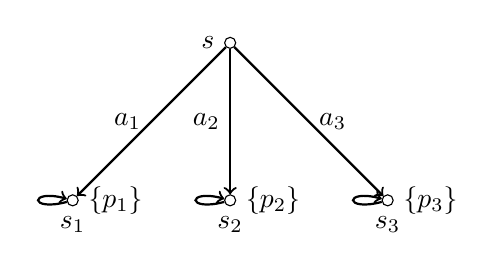
\begin{tikzpicture}
\node(-1) at (2,0) {};
\node[circle,draw=black, minimum size=4pt,inner sep=0pt,  label=left:{$s$}](1) at (0,0) {};
\node[circle,draw=black, minimum size=4pt,inner sep=0pt, , label=below:{$s_1$}, label = right:{$\{p_1\}$}](2) at (-2,-2) {};
\node[circle,draw=black, minimum size=4pt,inner sep=0pt, , label=below:{$s_2$}, label = right:{$\{p_2\}$}](3) at (0,-2) {};
\node[circle,draw=black, minimum size=4pt,inner sep=0pt, , label=below:{$s_3$}, label = right:{$\{p_3\}$}](4) at (2,-2) {};

\draw [->,thick](1) to node[left,align=left] {$a_1$} (2);
\draw [->,thick](1) to node[left,align=left] {$a_2$} (3);
\draw [->,thick](1) to node[right,align=left] {$a_3$} (4);
\draw [->,thick] (2) to [loop left]  (2);
\draw [->,thick] (3) to [loop left]  (3);
\draw [->,thick] (4) to [loop left]  (4);
\end{tikzpicture}
}
\caption{CGS $\G$ for a single agent. Labels for self-loops are omitted for readability.}
\label{fig::hardness}
\end{figure} 

\subsection*{Satisfiability}
The proof of undecidability of $\mathsf{SL}$ \cite{mogavero16} uses only the next-time fragment of $\mathsf{SL}$. Here we show how the proof can be adapted for the case of $\CSL$. For more details see the original proof in \cite{mogavero16}.

Given two variables $x_1$ and $x_2$, let $x_1 < x_2$ be the formula $\assign{x_1,y} p \land \assign{x_2,y}\neg p$. Define also $\varphi_{unbd}= \forall x_1 \exists x_2 (x_1 < x_2)$, $\varphi_{mn}= \exists x_2 \forall x_1 \neg (x_1 < x_2)$, and 
$\varphi_{trs}= \forall x_1 \forall x_2 \forall x_3 ((x_1 < x_2 ) \land  (x_2 < x_3 ))\imp (x_1 < x_3) $. Finally let 
    $\varphi_{<} =\varphi_{unbd}\land \varphi_{mn} \land \varphi_{trs}$. 

   \begin{proposition}
       Formula $\varphi_<$ is satisfiable.
   \end{proposition}
   \begin{proof}
       %For satisfiability. 
       Consider the $CGS$ $\G^\star$ with three states $s_0,s_1,s_3$, where $\Ac=\mathbb{N}$, and where we have that  $\tuple{s_0,k,j,s_1}\in R$ iff $k < j$, $\tuple{s_0,k,j,s_2}\in R$ iff $k\geq j$ and $\tuple{s_i,k,j,s_i}$ for $i=1,2$ and $k,j\in \mathbb{N}$. Moreover suppose that $\mathcal{V}(s_0)=\mathcal{V}(s_2)=\emptyset$ and $\mathcal{V}(s_1)=\set{p}$. It is easy to verify that $\G^\star,s_0 \models \varphi_<$. 
   \end{proof}

   In the proof of the fact that $\varphi_<$ is satisfiable, we constructed a model over an infinite number of actions. We can now show that we cannot do with less, i.e. every model of $\varphi_<$ necessarily possesses an infinite number of actions. 

   \begin{lemma}
       Let $\G$ be a $CGS$ whose set of actions is $\Ac$, and $s$ is one of its states. Define a relation $\prec \subseteq \Ac \times \Ac$ by $\tuple{a,b}\in \prec $ iff $\G,s\models x_1 < x_2[a/x_1, b/x_2]$. If $\G,s\models \varphi_{<}$, then relation $\prec$ is a strict partial order without the maximal element, and hence $\Ac$ is infinite. 
   \end{lemma}
   \begin{proof}
     That $\prec$ is transitive and unbounded immediately follows from the fact that $\G,s\models \varphi_<$. The fact that no maximal element exists for $\prec$ follows from the irreflexivity of $\prec$ %of this latter relation: 
     Indeed, suppose that $\tuple{a,a}\in \prec$ for some action $a$. This means that $\G,s\models \assign{a,b} p \land \assign{a,b}\neg p$ for some $b$, i.e., for the unique $s'$ s.t. $\tuple{s,a,b,s'}\in R$ we have  that $\G,s'\models p\ \land \neg p$, which is a contradiction. %clearly impossible.  
     Since $\prec$ is a strict partial order without maximal elements on $\Ac \times \Ac$, we directly obtain that $\Ac$ must be infinite. 
   \end{proof}


Define $a\equiv b$ iff neither $a\prec b$ nor $b\prec a$. It is easy to see that if $\G,s\models \varphi_<$, then $\equiv$ is an equivalence relation on the set of actions of $\G$. Let us denote by $[a]$ the equivalence class of $a\in \Ac$ generated by $\equiv$. We define a  relation $\prec^\equiv$ on equivalence classes of actions by putting $[a]\prec^\equiv [b]$ iff for every $a\in [a]$ and every $b\in [b]$,  $a\prec b$ holds. We can now show the following property of $\prec^\equiv$. %We can prove the following quite easily. 

\begin{lemma}
   Suppose that $\G,s\models \varphi_<$, then the relation $\prec^\equiv$ on the class of equivalence classes generated by $\equiv$ is a strict total order with the minimal element and no maximal element. 
\end{lemma}
\begin{proof}
    Transitivity, irreflexivity and the non-existence of a maximal element are immediate.   We show that $\prec^\equiv$ is total and admits a minimal element. For totality, we argue by contradiction: assume that $[a]$ and $[b]$ are two different incomparable equivalent classes. By definition, this means that there are $a,a'\in [a]$ and $b,b'\in [b]$ such that $a \not \prec b$ and $b'\not \prec a'$. This means that $b\prec a$ and $a' \prec b'$ must hold. Since $a$ and $b'$ are in different equivalence classes, %they must be comparable. W.l.o.g. 
    w.l.o.g. we can assume then that $a\prec b'$, which implies $b\prec b'$ by transitivity. But this is impossible since $b,b'\in [b]$. 
    
    Now suppose that there is no minimal element for $\prec^\equiv$. This implies that in $\G$ for every action $a \in [a]$ we can find an action $b \in [b]$ such that  such that $\G,s\models x_1 < x_2 [b/x_1, a/x_2]$ and thus $\G,s\models \forall x_2 \exists x_1 (x_1 < x_2)$. But this contradicts the conjunct $\varphi_{mn}$ of $\varphi_<$, i.e. $\G,s\models \exists x_2 \forall x_1 \neg (x_1 < x_2)$. 
\end{proof}
   
Having defined appropriate relations, we can use them to capture the construction of a tiling.
 Given a finite set $D$ of domino types and two relation $H,V\subseteq  D\times D$ the $\mathbb{N}\times \mathbb{N}$, \textit{the domino tiling problem} consist in finding a mapping $T: \mathbb{N}\times \mathbb{N} \to D$ such that for every $x,y\in \mathbb{N}$ it holds that $T(x,y)\in H$ implies $T(x+1,y)\in H$, and $T(x,y)\in V$ implies $T(x,y+1)\in V$. We can now use the reduction from the tiling problem to show the undecidability of the satisfiability problem for $\CSL$.
 %now show that this undecidable problem can be reduced to the satisfiability of a $\CSL$ formula. 

 
 Given $x_1$ and $x_2$, we define the two formulae $x_1 <_H x_2 = \exists y \assign{x_1,y} p \land \assign{x_2,y} \neg p$  and $x_1<_V x_2= \exists y \assign{y,x_1} p \land \assign{y,x_2}$. For $X\in \set{H,V}$, let $\varphi^X_{<}$ be defined symilarly to $\varphi_<$.
 Finally, let $\varphi_{grd}$ be the conjunction of $\varphi^H_<$ and $\varphi^V_<$. Intuitively, $\varphi^{grd}$ enforces the horizontal and vertical orderings of the positions in a grid.  Evidently, the sentence $\varphi^{grd}$ is satisfiable and every of its model has a countable number of actions. 
 
 By defining, for $X\in \set{H,V},$ $a\prec_X b$  similarly to $a\prec b$, we obtain that $\prec_X$ is a strict partial order with no maximal element on the set of actions on every model $\G$ of $\varphi^{grd}$. Let $\equiv_X$ for $X\in \set{H,V}$ be the equivalence relation on actions of $\G$ generated as $\tuple{a,a'}\in \equiv_X$ iff neither $a \prec_X a'$ nor $a'\prec_X a$. Then, by denoting $\Ac^\equiv_X$ the class of equivalence classes modulo $\equiv_X$, we get that $\prec^\equiv_X$ is a strict total order with the minimal element and no maximal element. Since $\Ac^\equiv_X$ is countable, it follows that $\tuple{\Ac^\equiv_X,\prec^\equiv_X}$ is a well-ordered set. We denote by $[a]^X_i$ the $i$-th element of $\Ac^\equiv_X$ w.r.t. $\prec^\equiv_X$. 
 
 Let $\mathcal{N}: \mathbb{N}\times \mathbb{N} \to \Ac^\equiv_H \times \Ac^\equiv_V$ be a mapping that maps any pair $\tuple{i,j}$ of natural numbers to the pair $\tuple{[a]^H_i, [a]^V_j}$.  
 We can define the successor relation %$S^X(x_1,x_2)$ as $(x_1 \prec_X x_2) \land \forall x_3 (\neg (x_3 \prec_X x_2) \land \neg (x_1 \prec_X x_3))$ 
 $S^X(x_1,x_2)$ as $(x_1 \prec_X x_2) \land \forall x_3 \neg((x_3 \prec_X x_2) \land (x_1 \prec_X x_3))$
 for $X\in \set{H,V}$. In such a way we ensure that if $\G,s\models \varphi_{grd}$ then $\G,s\models S^X(x_1,x_2)[a/x_1,a'/x_2]$ iff $a\in [a]^X_i$ and $a'\in [a]^X_{i+1}$. 
 
 Having defined the successor relation, we can now express the local compatibility of a tiling  $\varphi^{loc,t}$, i.e. that each tile has only one type, as well as horizontal and vertical requirements of a tiling $\varphi^{t,H}$ and $\varphi^{t,V}$.

 \begin{enumerate}
     \item $\varphi^{loc,t}= \assign{x,y}(t\land^{t'\neq t}_{t'\in D} \neg t')$
     \item $\varphi^{t,H}= \bigvee_{\tuple{t,t'}\in H} (\forall x (S^H (x,x') \imp \assign{x',y} t'))$
     \item $\varphi^{t,V}= \bigvee_{\tuple{t,t'}\in V} ( \forall y (S^V (y,y') \imp \assign{x,y'} t'))$
 \end{enumerate}

 Finally, let $\varphi^{tile}$ be $\forall x \forall y ( \varphi^{loc,t} \land \varphi^{t,H} \land \varphi^{t,V})$, and let the formula for the tiling problem be $\varphi^{dom}:= \varphi^{grd} \land \varphi^{tile}$. 

\begin{theorem} The satisfiability problem for $\CSL$ is undecidable. 
\begin{proof}
    To obtain the result one shows that there is a reduction from  the $\mathbb{N}\times \mathbb{N}$ tiling problem to the satisfiability problem of $\CSL$. Having defined all the necessary formulae above, the proof goes similarly to \cite[Theorem 3.10]{mogavero16}.
\end{proof}
    
\end{theorem}